\chapter{Outlook}
\label{chapter:outlook}

In this chapter we look beyond the diploma project and present our ideas about possible features.



\section{Hosting Documents on a Server}
Currently, if a user publishes a document, the server logic is hosted
in the same Java Virtual Machine (JVM) as the client application. We considered
this the most natural architecture. However, in some cases it might be
desirable to have a dedicated server machine that can host the server
logic instead of the publisher.

The server logic itself does not make any assumptions about the location
of the publisher. The publisher code may run inside the same JVM or it may run
on a different computer. It does not make any difference to the server logic.
Therefore, it would be relatively straightforward to create a standalone
document hoster, a server application that hosts published documents.

This would require some changes to the APIs. The following high-level
changes would be needed:

\begin{itemize}
 \item make \texttt{PublisherPort} and \texttt{PublisherConnection} part of the public API between the network and the collaboration layer
 \item add interfaces that allow the network layer to publish a document on a host (interface between collaboration and network layer)
 \item provide the application layer a way to specify where to publish the document (interface between application and collaboration layer)
\end{itemize}



\section{Network Simulator}
A simulated network layer would simplify testing of both the collaboration as 
well as the network layer. Therefore, creating a simulated network layer
will be one of the first things we will do. A simulated network layer
consists of a custom implementation of the network layer interfaces. Possible 
features for such a simulated network layer include:

\begin{itemize}
 \item simulate connection failures
 \item simulate slow connections
\end{itemize}

The idea is to have the possibility to start several instances of the
application inside the same JVM. These instances represent distinct users.
By switching between these users, the application and collaboration layer
could be tested without accessing the network.



\section{Improved Access Control}
ACE has a very rudimentary access control. Each user that wants to join a
session needs the approval of the publisher. Once he is part of the session
he has full read-write access. Alternatively we could add a read-only
access mode. A user in read-only access mode cannot write anything in
the session, but he sees all the changes.

Adding a read-only access mode would need some changes to all layers of
the application:

\begin{itemize}
 \item support assigning access rights to a user by the publisher
 \item notify all participants about their access rights as well as about
       the access rights of the other participants
 \item enforce the access rights in the server logic
\end{itemize}

Some interesting issues need to be resolved before this feature can be
implemented. First, if the publisher changes the access rights of a 
participant, this change has to be sent to the other participant. In the
meantime that participant still sends requests to the server logic. The
question arises, at which moment the new access rights should be enforced.
If the access rights are enforced right from the moment where the publisher
assigns the rights, some requests from the participant might be rejected by the 
server. However, the operations of the request have already been applied
to the participant's document. Therefore, the participant would have to
be notified about these rejected requests and would have to undo their
effect on the local document.



\section{User Authentication with Digital Signatures}
A very interesting addition would be the use of digital signatures to help
the user decide who should be allowed to join. By using digital
signatures, the user could be confident about the identity of joining users.
However, we think that this feature should not sacrifice the simplicity
of the application. It should be possible to support standard certificates
as well as PGP (Pretty Good Privacy) certificates.


\section{Peer to Peer Communication}
Explicit user discovery makes it possible to connect to users that are outside 
of the local area network. Consider the following figure:

\begin{figure}[H]
 \centering
  \frame{
 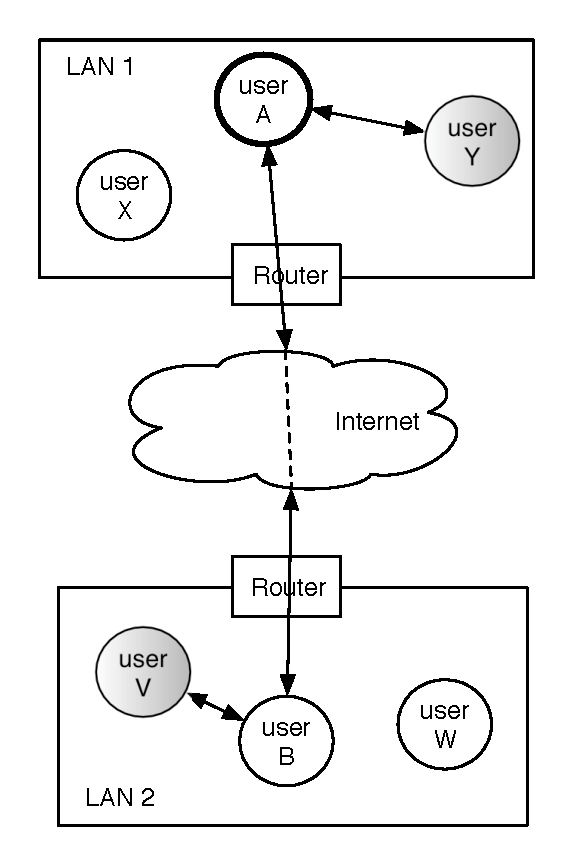
\includegraphics[width=3.60in,height=5.54in]{../images/finalreport/outlook_peerToPeer.eps}
 }
 \caption{Use peers as proxies to overcome routers or firewalls (e.g. \emph{V} connects to \emph{W})}
 \label{fig:outlook.peertopeer}
\end{figure}

User A from within network 1 published a document and user Y joined it. User A then explicitly discovers user B in network 2 (router for LAN 2 not restrictive). The two users are connected via the Internet. If the user B then joins a shared document from user A and other participants reside inside the local area network 1 (user Y), user B will be notified about these users too and vice versa. If network 2 also hosts more users, the discovery process could continue this way. The system then becomes similiar to a peer-to-peer system. Especially the following problem could be interesting to solve using a peer-to-peer like architecture: One problem that could arise is with firewalls or routers that block application ports between networks. Lets say router for LAN 1 is restricitve and blocks incoming connections. Now user B wants to join a document published by user Y (user B knows of user Y and his documents because of the participation in the document session of user A). User B cannot directly connect to user Y since the router for LAN 1 blocks it. To bypass these barrier, user B could user A as a proxy to connect to user Y.
Another scenario could be that user V wants to invite user Y to join his document and use user B in LAN 2 and user A in LAN 1 as proxies to connect to user Y. 

Many interesting issues (such as using other users as proxies) arise that could be implemented in the future. Also, the need for a thorough document access control and user authentication intensifies when proxy functionality comes into play and users from everywhere could join a document.

Currently, the implementation does not support the use of proxies. If a firewall or a router blocks the connection,  the discovery or the join request simply fails.